\documentclass[11pt]{article}
\usepackage{fontspec}
\usepackage{enumitem}
\usepackage{amsmath}
\usepackage{amssymb}
\usepackage{eurosym}
\usepackage[english]{babel}
\usepackage[letterpaper]{geometry}
\usepackage{xcolor}
\usepackage[font=footnotesize]{caption}
\usepackage{url}
\usepackage{natbib}
\usepackage{bibentry}
\usepackage{framed}
\usepackage{xspace}
\usepackage{changepage}
\usepackage[framemethod=TikZ]{mdframed}
\usepackage[font=footnotesize]{subcaption}
\geometry{verbose,tmargin=2cm,bmargin=3cm,lmargin=2.5cm,rmargin=2.5cm,headheight=.5cm,footskip=1.5cm}

\nobibliography*

\newenvironment{mybox}[2][]{%
\ifstrempty{#1}%
{\mdfsetup{%
frametitle={%
\tikz[baseline=(current bounding box.east),outer sep=0pt]
\node[anchor=east,rectangle,fill=blue!20]
{\strut};}}
}%
{\mdfsetup{%
frametitle={%
\tikz[baseline=(current bounding box.east),outer sep=0pt]
\node[anchor=east,rectangle,fill=blue!20]
{\strut #1};}}%
}%
\mdfsetup{innertopmargin=10pt,linecolor=blue!20,%
linewidth=2pt,topline=true,%
frametitleaboveskip=\dimexpr-\ht\strutbox\relax
}
\begin{mdframed}[]\relax%
\label{#2}}{\end{mdframed}}


\setlength{\parindent}{0pt}
\setlist{nolistsep,noitemsep}
% \setlist{leftmargin=*}
\setlength{\parskip}{\medskipamount}
\setlength{\itemsep}{1pt}
  \setlength{\parsep}{0pt}
  
\definecolor{gray75}{gray}{0.75}
\definecolor{gray50}{gray}{0.50}
\definecolor{formalcolor}{gray}{0.9}
\definecolor{formalshade}{rgb}{0.95,0.95,1}


\renewcommand\thesubfigure{\alph{subfigure}}
\newcommand{\hsp}{\hspace{0.2em}}
\newcommand{\comment}[1]{\textcolor{green!60!black}{\sffamily [\textit{#1\dots}]}}
\newcommand{\com}[1]{\textcolor{red!60!black}{\sffamily [\textit{#1}]}}

\newcommand{\eg}{\textit{e.g.},\,}
\newcommand{\ie}{\textit{i.e.},\,}
\newcommand{\etal}{\textit{et al.}\xspace}
\setlength{\bibsep}{6pt plus 0.3ex}

\makeatletter
%%% Custom sectioning (titlesec package)
\usepackage{titlesec}
\titleformat{\section}%
  [hang]% shape
  {\normalfont\Large\itshape}% format applied to label+text
  {\llap{\hspace*{-20pt}\thesection\hsp\textcolor{gray50}{|}\hsp}}% label
  {0pt}% horizontal separation between label and title body
  {}% before the title body
  []% after the title body

\renewcommand{\maketitle}{%
  \begingroup
  \setlength{\parindent}{0pt}
  \setlength{\parskip}{6pt}
  \linespread{1.1}
    {\begingroup
      \sffamily
	  \par{\Huge\uppercase{\@title}}
      \par{\@author}
      \par
%      \vspace*{0.5cm}
%      \textbf{\sffamily Date:} {\@date}
    \endgroup}
  \endgroup
}
\renewcommand\thefigure{\arabic{figure}}
\captionsetup[figure]{labelfont=bf,labelsep=period}
\renewcommand\thesubfigure{\alph{subfigure}}
\setlength{\bibsep}{6pt plus 0.3ex}
\newenvironment{formal}{%
  \vspace*{-5pt}
  \def\FrameCommand{%
    \hspace{-5pt}%
    {\color{gray50}\vrule width 1.25pt}%
    \colorbox{formalcolor}%
  }%
  \MakeFramed{\advance\hsize-\width\FrameRestore}%
  \noindent\hspace{-4.55pt}% disable indenting first paragraph
  \begin{adjustwidth}{}{7pt}%
  \normalsize
  \vspace{-2pt}
}
{%
  \vspace{2pt}\end{adjustwidth}\endMakeFramed%
  \vspace*{-10pt}
}

\makeatother
 
%This is ShareLaTeX Specific (or if the fonts are not installed in your system)
%-----------------------------------------------------------------------
% Times New Roman
\setromanfont[
Path=./fonts/,
BoldFont=MinionPro-Bold.otf,
ItalicFont=MinionPro-It.otf,
BoldItalicFont=MinionPro-BoldIt.otf,
]{MinionPro-Regular.otf}
% Arial
\setsansfont[
Path=./fonts/,
BoldFont=HelveticaNeueLTPro-Md.otf,
ItalicFont=HelveticaNeueLTPro-LtIt.otf,
BoldItalicFont=HelveticaNeueLTPro-MdIt.otf
]{HelveticaNeueLTPro-Lt.otf}
% Courier New
\setmonofont[
Path=./fonts/,
Scale=0.90,
BoldFont=courbd.ttf,
ItalicFont=couri.ttf,
BoldItalicFont=courbi.ttf
]{cour.ttf}
%-----------------------------------------------------------------------
 
\title{Réponse aux rapporteurs}

%\date{\today}

\begin{document}
 
\maketitle

\def\baselinestretch{1.1}
\normalsize

\vspace{10pt}

\textit{Je tenais à remercier Marco Fiore et Sidi-Mohammed Senouci pour avoir pris le temps de lire ma thèse avec détail et rédigé leurs rapports qui, par leurs commentaires très pertinents m'ont donné des éléments de réflexion par rapport à mon travail. Ce document résume les motivations des changements que j'ai effectués pour la version finale de mon manuscrit suite aux commentaires des rapporteurs.}

\section{Chapitre 1}

\begin{formal}
    \textbf{(Marco Fiore).} In particular, the motivation for the work could be better supported: there is no incontestable evidence that there exists a need to extend the wired network capacity to accommodate the existing or future traffic demand, or that there is an economic advantage for the service or network provider in offloading some traffic to a vehicle-based system.
\end{formal}

Je vous remercie pour avoir pointé le manque de motivations. Le besoin d'une telle infrastructure de délestage découle du fait de l'augmentation de la demande pour du trafic IP, jusqu'à atteindre parfois la limite de la capacité des fournisseurs d'accès à Internet.

De ce fait, j'ai ajouté la phrase suivante au troisième paragraphe de la section~1.1 (\textit{Context}) afin de motiver le besoin d'une telle infrastructure de délestage~:
\begin{quote}
With data-intensive applications such as high-definition video, autonomous vehicles, and virtual reality, the demand for network bandwidth grows by an estimated 22\% per year. Already the case in some situations, in the next few years, the data consumption will outpace the network improvements made by providers in laying high-capacity fiber and speeding up their already-existing network infrastructure and servers~\cite{hecht2016bandwidth}. As shown in Figure~1.1, the demand for bandwidth is at its strongest today: global IP traffic has grown threefold during the past six years and is expected to double within the five next years~\cite{index2014forecast,gantz2012digital}.
\end{quote}

J'ai également ajouté la phrase suivante au premier paragraphe de la section~1.2 (\textit{Vision and data offloading design}) pour montrer l'importance du trafic d'arrière plan par rapport à la part du trafic IP global~: 
\begin{quote}
As noted by Hecht, the synchronization of the private content between remote data centers is one of the biggest drivers of bandwidth demand~\cite{hecht2016bandwidth}.
\end{quote}

\begin{formal}
    \textbf{(Marco Fiore).} Also, given the originality of the proposed scenario, examples of how a vehicle-based offloading system could enable viable business models would have made the discussion stronger.
\end{formal}

Il est vrai que présenter un \textit{business model} renforce la force de la proposition. C'est pourquoi j'ai ajouté des phrases au cinquième paragraphe de la section~1.1 (\textit{Context}) lorsque je mentionne des services à valeur ajoutée tels que UberRUSH ou Greyhound~:

\begin{quote}
In our case, private vehicles transport data for the account of content providers in exchange for their normal routine (\eg to synchronize backup data between remote data centers they operate). A service provider is then in charge of supervising the offloaded transfers then charged to the content providers and providing incentives to the vehicle owners for the data they transport (\eg through a ``get paid to drive'' program).
\end{quote}

Par ailleurs, j'ai ajouté la figure suivante (numérotée~\ref{fig:business-model} dans ce document et 3.2 dans la nouvelle version du manuscrit) à la section~3.1.2 (\textit{Business model, assumptions, and roles}) du chapitre~3 où l'on décrit les différents acteurs et leur rôles respectifs dans le délestage de données.

\begin{figure}[h!]
    \centering
    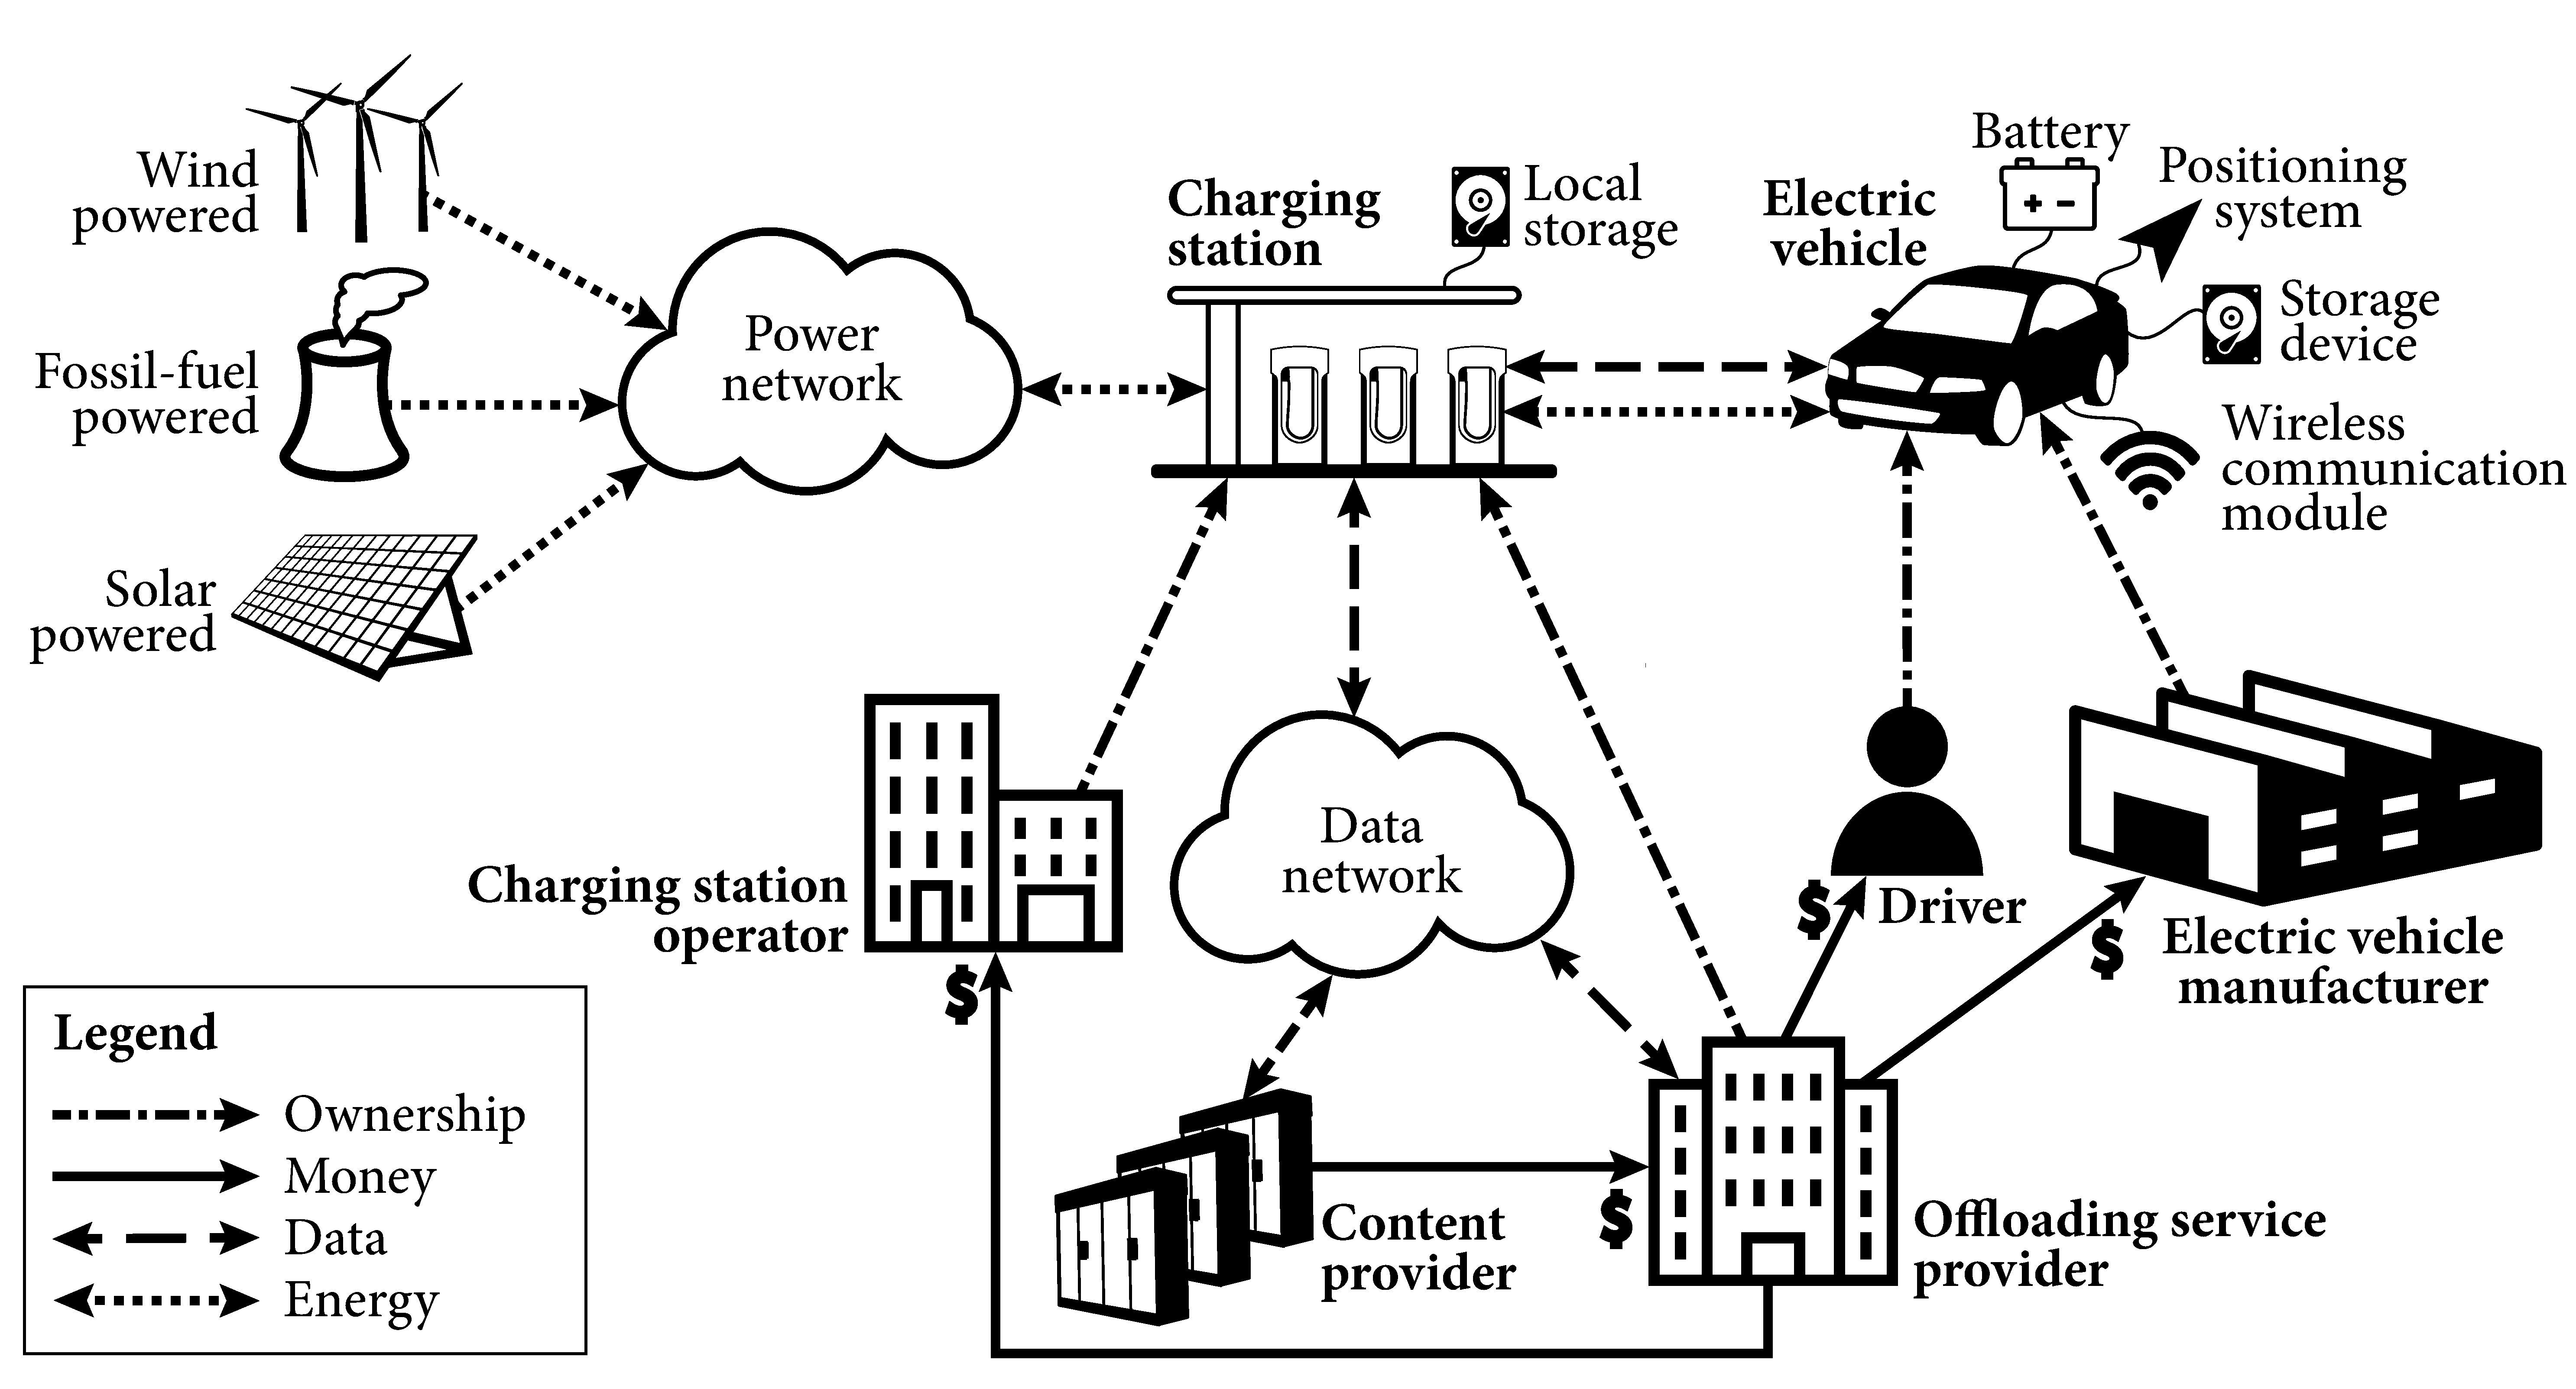
\includegraphics[width=0.9\textwidth]{figures/business-plan.pdf}
    \caption{Business model for the vehicular data offloading concept.}
    \label{fig:business-model}
\end{figure}

\begin{formal}
    \textbf{(Marco Fiore).} Finally, drivers’ and passengers’ privacy risks are not mentioned, although these are critical aspects in a system that assumes the sharing of positioning data and the prediction of future trajectories of individual users.
\end{formal}

Il est vrai qu'il serait mieux d'introduire dès le début les problèmes de protection de lq vie privée liés à l'utilisation des données de positionnement des véhicules. C'est pour cette raison que j'ai choisi de présenter un plan de la thèse par chapitre et des différentes discussions qui leur sont associées dans un paragraphe (\textit{Thesis outline}) de la section~1.4 (\textit{Contributions and thesis outline})~:
\begin{quote}
 This manuscript is organized in six chapters, including this introduction (Chapter~1). Chapter~2 presents a review of previous approaches that propose to use mobility of entities to transport data. The two following chapters~3 and~4 present the main contribution of the thesis with, respectively, a revenue analysis and a practical implementation of the vehicular data offoading system. Chapter~5 presents two extensions of the data offoading system for vehicular cloud services. Each chapter begins with a brief introduction followed by a list of the main contributions. Given the novelty of our work, we provide additional discussions for each chapter on related topics we chose not to address in detail, including data security, privacy con- cerns, and road traffc dynamics. Finally, we conclude this thesis with a last chapter (Chapter~6) that summarises our work and a raises futher questions as a plan for future research.
\end{quote}

\section{Chapitre 2}

\begin{formal}
    \textbf{(Marco Fiore).} However, the taxonomy lacks some form of comparative assessment that clearly identifies the advantages and disadvantages of each technique and allows pinpointing the current state-of-the-art~---~against which the proposed system could be compared.
    
    Also, the discussion is limited to in-network data transfers, while physical mobility-based solutions for content download and upload, or for infrastructure planning are overlooked despite being quite relevant to the thesis work.
\end{formal}

J'ai changé la section~2.3 (Relevance to the thesis) pour faire dans un premier temps un résumé des différentes approches similaires à notre approche de délestage des données (au niveau du paragraphe 
\textit{Vehicular data offloading}). Dans un second temps, j'ai ajouté les travaux relatifs aux deux extensions que nous proposons au niveau du paragraphe \textit{Vehicular cloud services}. Enfin, j'ai conservé les deux derniers paragraphes (\textit{Logical view of the vehicle movements} et \textit{Centralized architecture}) qui regroupe des concepts transversaux aux approches relatives à notre approche.

\begin{quote}
\noindent\textbf{Vehicular data offloading.} 
In the first part of our work, we rely on offloading spots that act as intermediate relay nodes similar to those used to asynchronously compose entity trajectories at pre-defined locations such as throwboxes~\cite{zhao2006capacity}. In this case, these intermediary nodes create additional contact opportunities and bring the data closer to its destination. They also introduce non-randomness in an environment where entity trajectories are difficult to predict. The authors showed that these nodes are an effective way to compose the entity trajectories and improve the overall throughput and delivery delay.

Our system aims to transfer large amounts of delay-tolerant data, between remote locations. Examples of large data transfers over the Internet range from exchanges of large scientific datasets to distribution of high-resolution movies. Some protocols have been developed to handle bulk data transfers of several Terabytes per day, such as GridFTP~\cite{allcock2003gridftp} or NetStitcher~\cite{laoutaris2011inter}. The latter takes into account unused bandwidth in inter-data center networks (during low link utilization periods) by using multi-path and store-and-forward scheduling at intermediate nodes for bulk transfers.

While these previous approaches allow transferring bulk data, we propose to \textit{physically offload} data by creating an alternative communication channel consisting of existing vehicle movements. Several works proposed to create such a channel by relying on the movements of entities such as airline passengers~\cite{keranen2009dtn}, trains~\cite{zarafshan2010trainnet}, or even postal services~\cite{wang2004turning,cho2011budget,laoutaris2013delay}. While these approaches are comparable with our work in terms of scale, throughput, and delay, they are difficult to compare under equivalent settings, including the number of entities involved and trips made, as well as their coverage.

\noindent\textbf{Vehicular cloud services.}
In the case of the first extension, we rely on the schedule movements of public buses to distribute user files among repositories. This work is closely related to KioskNet~\cite{seth2006low} and DakNet~\cite{pentland2004daknet}, although they do not provide any performance evaluation and they take place in rural environments with fewer bus routes and trips available. In our system, the bus act as message ferries that connect the repositories together~\cite{zhao2004message}. While they are not controllable, they have the same purpose to connect remote nodes together.

The consumer/producer behavior of the mobile users is similar to the TierStore system, which acts as a Network File System (NFS) for applications with limited bandwidth or a challenged network environment~\cite{demmer2008tierstore}. User files are stored in persistent storage repositories that lie at the core of the system (\ie static nodes similar to our repositories). Updates are applied locally at the persistent repository and distributed to other nodes. The system also uses the movements of mobile nodes to distribute updates to and from the nodes using static multicast. On the other hand, Ott and Pitk{\"a}nen proposed to use the mobile nodes to temporarily store content by means of caching~\cite{pitkanen2007redundancy,ott2007dtn} to decrease the latency when retrieving a content. This approach is similar to the one proposed by Haggle, a \textit{Pocket Switching Networking} (PSN) system that enables caching of content at intermediate nodes to also reduce the delivery delay~\cite{scott2006haggle}.

The placement of the repositories in this extension is similar to the placement of throwboxes \cite{zhao2006capacity}, where the authors select the optimal locations for throwboxes from a set of candidate locations (\ie centers of square cells dividing the geographical space) to maximize the total data rate, given different knowledge on contact opportunities and traffic load for various routing strategies (\ie single-path, multi-path, and epidemic). However, our placement does not account for the routing strategy, which makes it more related to the one proposed by Chawathe in the context of dead drops to disseminate data~\cite{chawathe2006inter}. In this case, the drop boxes have the same behavior as our repositories and data is disseminated using the (known) movements of vehicles. The placement of dead drops must provide the required connectivity among them at minimum deployment cost and is solved using a heuristic of the minimum-weight $k$-set cover problem fitting the model.

Finally, in the second extension, we leverage pre-defined locations selected such that vehicles encounter for a duration long enough to transfer large amounts of data through vehicle-to-vehicle communications. While these locations are similar to those used for wireless switching by Tan~\etal to create a ``vehicular backbone network''~\cite{tan2014vehicular}, or those used by Sarafijanovic-Djukic \etal to perform data forwarding~\cite{sarafijanovic2006island}, our work studies the capacity of the contacts at specific locations.
\end{quote}

\begin{formal}
\textbf{(Marco Fiore).} Less convincing is the modeling of the data traffic demands and of the costs of data transfers with the traditional and vehicle-based techniques, which is fairly arbitrary in all cases.
\end{formal}

Les demandes de trafic sont générées arbitrairement par des fournisseurs de contenus et caractérisées par une quantité de données à transférer en un temps imparti avec un taux de perte maximum. Nous avons fait le choix arbitraire d'exprimer le coût d'un transfert de données en fonction de la distance entre la source et la destination du transfert. J'ai ajouté une figure (figure~\ref{fig:demand-price-km} dans ce document et figure~3.8 dans le manuscrit) paragraphe à la section~3.5.5 (\textit{Revenue maximization of offloading data}) pour illustrer ce coût et son comportement en fonction de la distance de la source à la destination.

\begin{figure}[h!]
    \centering
    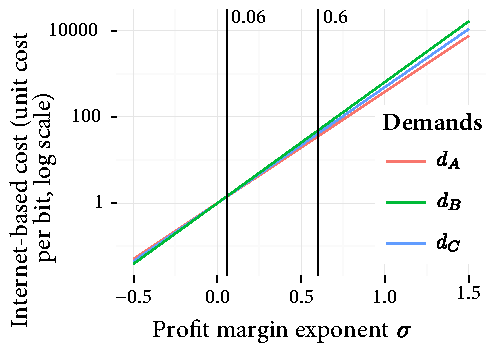
\includegraphics[width=7.2cm]{results/ton-demand-price-km.pdf}
    \caption{Internet-based cost (expressed as the unit cost per bit transferred) as a function of the profit margin exponent for each demand $d_A$, $d_B$, and $d_C$.}
    \label{fig:demand-price-km}
\end{figure}

\begin{quote}
We represent the Internet-based cost $\gamma_{st}$ to transfer a bit of data as a function of the profit margin exponent $\sigma$ for each demand $d_{st}\in\{d_A,\,d_B,\,d_C\}$ in Figure~\ref{fig:demand-price-km}. As shown in the figure, the Internet-based cost increases with the distance (\eg it is greater for the furthest demand $d_C$) for positive values of the profit margin exponent. Note that the Internet-based cost can be adjusted with a factor to account for more realistic prices.
\end{quote}

\begin{formal}
\textbf{(Marco Fiore).} Moreover, the choice of not showing results on the revenue is questionable, since the optimization problem aims at maximizing precisely that measure. These results are also important to understand if (and under which cost parameters) there is an advantage in offloading data to a vehicle-based system~---~which remains an open question.
\end{formal}

J'ai ajouté à la section~3.5.5 (\textit{Revenue maximization of offloading data}) des résultats (figure~\ref{fig:revenue-delay-tolerance} dans ce document et figure~3.11 dans le manuscrit) et leurs explications concernant les revenus de l'utilisation du système de délestage de données sur le réseau routier. À noter que les coûts exprimés sont unitaires par bit transporté et peuvent être modulés à l'aide d'un facteur. 

\begin{figure}[h!]
\centering
    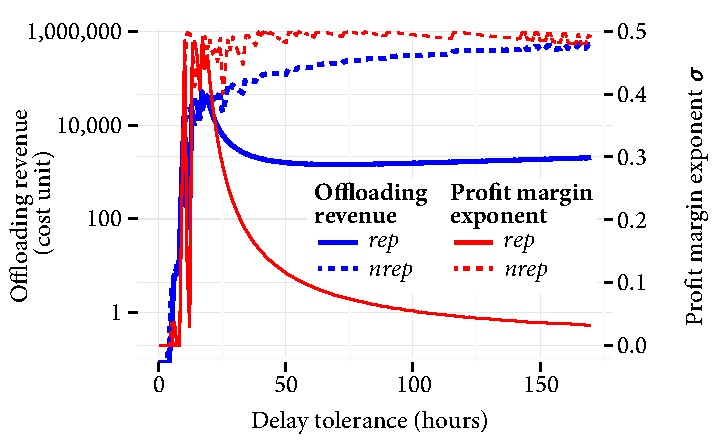
\includegraphics[width=8.2cm]{results/revenue-delaytolerance.pdf}
    \caption{Offloading revenue as a function of the delay tolerance resulting from the allocation of demands $d_A$, $d_B$, and $d_C$, respective to Figure~3.9b.}
    \label{fig:revenue-delay-tolerance}
\end{figure}

\begin{quote}
We represent the offloading revenue (in terms of cost unit) for the allocations of demands $d_A$, $d_B$, and $d_C$ (respective to Figure~3.9a as a function of the delay tolerance of the offloading demands. Note that the revenue depends on the Internet-based cost and the profit margin exponent $\sigma$. Recall that the latter is chosen for each allocation of the demands given a delay tolerance to guarantee fair allocation of the demands, such that it minimizes the standard deviation of the mean throughput resulting from the allocation of the demands. For this reason the resulting offloading revenue is unstable for small delay tolerances (\ie < 50 hours). When increasing the delay tolerance of the offloading demands, the profit margin decreases to guarantee the fairness of the allocations of the demands and the revenue increases. Since more data is transferred, the revenue is becoming less sensitive to the transfer distances and $\sigma$ decreases. Additionally, the revenue resulting from the \textit{rep} model is less than the \textit{nrep} model, as the operational costs when traversing the offloading spots are 1,000 times less for the \textit{nrep} model (since it requires less data to be stored temporarily due to replications).
\end{quote}


\section{Chapitre 4}

\begin{formal}
\textbf{(Sidi-Mohammed Senouci).} Je trouve ce chapitre réussi mais manque des discussions sur les limites de la solution (protection de la vie privée vu que les conducteurs vont partager des informations sur leurs destinations, la dynamique du trafic pendant la journée/semaine/saison). Ceci n’altère en aucun cas la qualité de la proposition et le souci du détail dans la mise en place de la solution qui est extrêmement appréciable.
\end{formal}

Je vous remercie pour cette remarque pertinente. Puisque le système d'allocation considère seulement des comptages de trafic moyennés sur une année, il serait en effet intéressant de discuter l'utilisation de comptages de trafic avec une granularité plus fine. A cet effet, j'ai ajouté la discussion suivante (section~4.5.1, \textit{On the choice of traffic counts}) au chapitre~:

\begin{quote}
\noindent\textbf{Annual Average Daily Traffic}
The purpose of our performance evaluation is to assess the capacity enhancement brought to the Internet by the road network. Our evaluation aims at determining the amount of data that can be transferred on the road within a given time period. A typical transfer lasts from a few days to a week, as we can offload up to one Petabyte. The traffic counts we use are provided by the AADT (\textit{Annual Average Daily Traffic}), which are yearly averages. As so, AADTs average out the effects of seasonal and diurnal variations or missing data due to flawed monitoring. To determine the traffic volume of a road segment over the duration of a transfer, we multiply the corresponding AADTs by the transfer duration measured in days. The use of the AADTs prevents our evaluation results from being affected by the diurnal, seasonal, or flawed bias. 

To transpose our work in a practical setting or commercial use, thinner-grained traffic count averages should be used to account for transfers lasting few hours or several weeks. An established practice for inferring traffic count averages for different time periods consists in using temporal allocation factors applied to the annual AADTs. 

An example of temporal allocation factors can be found in ``The Traffic Monitoring Guide'' where they are referred to as \textit{group factors}. These factors are provided by the US Federal Highway Administration to help State Department of Transportation plan their local Highway Performance Monitoring System~\cite{wright1997variability,guide2013us}. The guide describes how to calculate the factor groups (\ie temporal allocation factors) from the traffic data collected. The procedure depends on the location and the characteristics of the road segment, as well as the time period of interest. The traffic assignment models presented in this paper remain pertinent and can be used in combination with the temporal allocation factors.

The factors resulting from this procedure are applicable for time periods of several months (seasonal), days (day-of-week), or hours. These factors determine the road traffic pattern as a ratio of the AADT for given road segments. The hourly vehicle volume $V_{i,\,t}$ on a road segment $i$ at time $t$ is estimated as the product of the average daily traffic $\textrm{AADT}_{i}$ and monthly $M_{g(i),\,t}$, daily $D_{g(i),\,t}$ and hourly $H_{g(i),\,t}$ factors, each for the factor group $g(i)$ of the road segment $i$:
\begin{equation}
    \label{eq:traffic-variation}
    V_{i,\,t} = \textrm{AADT}_{i} \times M_{g(i),\,t} \times D_{g(i),\,t} \times H_{g(i),\,t}.
\end{equation}
Note that the hourly factor takes into account the $D$-factor and the $K$-factor (directional and peak hour factors, respectively).

\noindent\textbf{Finer-grain traffic counts.}
Another way to carry out the study of a dynamic system with finer-grain traffic counts (\eg in the order of the hour or for 15-minute intervals) is to characterize the dynamic flows of vehicles between offloading spots. Numerous works from transportation research have studied the estimation and prediction of dynamic origin-destination matrices using traffic counts, in particular, Bierlaire and Crittin or Casetta \etal both propose to do so using sequential estimator (namely Generalized Least Squares)~\cite{bierlaire2004efficient,cascetta1993dynamic}. With dynamic origin-destination flows between the offloading spots, one can use the recent work~\cite{fleischer2007quickest} that built on Ford and Fulkerson~\cite{ford2015flows} to study the allocation of flows over time using time-expanded graphs. 
\end{quote}

De la même manière, il est important de considérer des problèmes liés à la protection de la vie privée des conducteurs qui doivent partager leurs informations de géo-localisation pour que le système puisse déterminer le prochain point de délestage auquel ils vont s'arrêter. De ce fait, j'ai ajouté une discussions sur les problèmes de protection de la vie privée des conducteurs à la discussion existante (section~3.6.3, \textit{Predicting the future direction of the stopping vehicles and privacy concerns}) du chapitre~3 sur la prédiction de la future trajectoire des véhicules lors de leurs arrêts aux points de délestage.

\begin{quote}
In order to \textit{accurately} predict the future offloading spot the vehicle will visit, the offloading service requires access to the positioning data of the vehicles, which raises some privacy concerns. While it is common for car manufacturers to collect and analyze such data (\eg Tesla collects the current location of the vehicles for remote vehicle analysis\footnote{https://www.tesla.com/about/legal}), we are aware of the privacy breach this represents for both the driver and passengers. In Section~3.1.2, we presented a ``get paid to drive'' program offered by the offloading service provider to the vehicle owners in exchange for transporting a storage device. With this incentive, some drivers may be more willing to share their positioning data with the service.  Otherwise, the offloading service provider could use the historical visit of the vehicle at charging stations (operated by the charging station operator) to infer the vehicles' future visits based on probabilistic tools (\eg Markov chains).

When the drivers do not want to share any data at all with the offloading service, the offloading spots discard the vehicles that do not share their positioning data because there is no means to predict where they will go next. In this case, these vehicles should not be involved in the data offloading.
\end{quote}

\begin{formal}
\textbf{(Marco Fiore).} Including information on the complexity and scaling properties of the centralized algorithm could further improve the discussion.
\end{formal}

Je vous remercie pour ce commentaire. Il est vrai que la complexité de l'algorithme n'a pas été mentionnée. C'est pourquoi j'ai ajouté un paragraphe à la fin de la section~4.3.2 (\textit{Max-min vehicle flow allocation model}) détaillant la complexité de l'algorithme.

\begin{quote}
The max-min fair allocation model presented in this section has a polynomial time-complexity because fractional flows are allowed in the linear programming models formulated in function \textsf{MCF} and the non-blocking algorithm~\cite{karakostas2008faster}. The time-complexity of both linear programming models grows in linear time with the number of demands and the number of paths in $\mathcal{P}_{st}$ for each demand $d_{st}$ of the set of demands to allocate.
\end{quote}

\section{Chapitre 5}

\begin{formal}
\textbf{(Sidi-Mohammed Senouci).} Il aurait été intéressant de discuter plus les motivations d’une réplication vers ‘tous’ les points de stockage, du nombre optimal de points à déployer et non seulement leur placement selon la dynamique du trafic.
\end{formal}

Ce sont en effet deux points qui manquent de clarté. J'ai ajouté un paragraphe à la section~5.1.1 (\textit{Problem statement}) motivant la réplication de l'utilisation de la réplication vers tous les points de stockage~:

\begin{quote}
While replicating files to all the repositories is inefficient in terms of file storage, it fits with our assumption of atomic contacts and unlimited file storage at the users and at the repositories. We further assume no locality bias with respect to where files are generated. Additionally, we assume that we cannot predict the trajectory of the mobile users, in particular, we cannot predict the sequence of storage nodes the mobile users will visit in the future. Under these assumptions, replicating files to all the repositories is the most straightforward approach to increase the availability of files and improve the success ratio of \texttt{get} requests.
\end{quote}

Par ailleurs, j'ai ajouté des discussions à la fin de ce chapitre (section~5.3, \textit{Discussions}) pour discuter des différentes politiques de réplications dans le cas où les contacts entre les stations de bus et les bus n'étaient pas atomiques. Cette discussion est accompagnée de la figure~~\ref{fig:allput-backend} dans ce document et figure~5.10 dans le manuscrit.

\begin{figure}
    \centering
    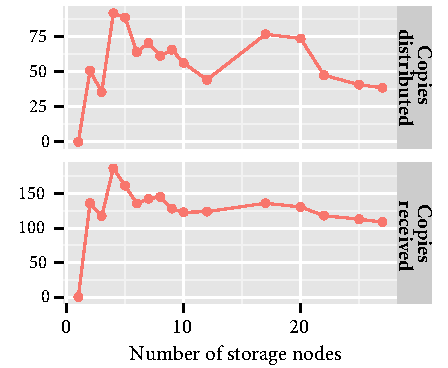
\includegraphics[width=6.5cm]{figures/allput-backend.pdf}
    \caption{Average number of copies distributed and received by the repositories for a file and a user request deadline of 2400~seconds.}
    \label{fig:allput-backend}
\end{figure}

\begin{quote}
\noindent\textbf{Replication strategies (first extension).} With the replication of file copies to every repository, a large number of copies is distributed and received by the repositories, as we show in Figure~\ref{fig:allput-backend}. With non-atomic contacts, we need to limit the overhead of copies sent over contacts between mobile users and repositories. With no knowledge of the future trajectories of mobile users, one could distribute copies of files for a bounded duration until the distribution of copies of the file stops. Alternatively, one could bound the number of copies generated per repository and transmitted to the mobiles users. With techniques borrowed from Delay Tolerant Networks, one could use a control plane that would enable the repositories to ``learn'' the frequent repositories the mobile users encounter along their route~\cite{lindgren2003probabilistic,grossglauser2006locating}. With this information, a single copy would be needed to transmit per repository.
\end{quote}

Concernant le nombre optimal de points de stockage à déployer, ce nombre est atteint une fois que toutes les demandes ont été allouées à stations de bus candidates. Afin de clarifier ce point, j'ai ajouté la phrase suivante dans la section~5.1.3 (\textit{Real experiment simulation})~:
\begin{quote}
For each simulation, we deploy a target number of repositories up until the optimal number of repositories, where no demands are left unallocated. 
\end{quote}

\begin{formal}
\textbf{(Marco Fiore).} These studies are less complete and conclusive than those on the main vehicle-based offloading system, and are characterized by stronger assumptions (\eg atomic contacts in the first extension) or reduced detail in the mobility representation (\eg undefined interpolation of GPS traces in the second extension).
\end{formal}

Il est vrai que ces extensions sont moins aboutie et complètes par rapport au travail principal du délestage de données, puisque ce sont des travaux préliminaires qui nécessitent d'être approfondies. Cependant, j'ai ajouté une discussion (paragraph \textit{Atomic contacts (first extension)}) à propos des contacts atomiques dans la section~5.3 (\textit{Discussions}).

Concernant les interpolations des traces GPS pour la seconde extension, j'ai ajouté des informations additionnelles expliquant la méthode utilisée au paragraphe \textit{Experimental setup} de la section~5.2.2 (\textit{Experimentation with a bus system}).

\begin{quote}
We used a recent map-matching algorithm proposed by Newson and Krumm to match the sequence of timestamps positions with the planned route given in the GTFS feed provided by the Dublin City council~\cite{newson2009hidden}. This step allowed us to remove outliers from the simulation, which could bias the results, as well as form more realistic trajectories by adding waypoints corresponding to the respective routes followed by the buses.

\begin{center}
[\dots]
\end{center}

The ONE can use real-world mobility traces to reproduce the movements of DTN nodes \textbf{using linear interpolation between two timestamped waypoints and infer their contacts}.
\end{quote}

\begin{formal}
\textbf{(Marco Fiore).} Also, in both extensions, the service use cases are not as sound as that underlying the work presented in the previous two chapters.
\end{formal}

Il est vrai que chacun de ces deux services manquent de motivations, comparé au service de délestage de données de la première partie. De ce fait, j'ai ajouté des éléments motivant leur déploiement lorsqu'ils sont introduits. Les changements sont notés en gras.

\begin{quote}
In the first section of this chapter, we exploit the storage capabilities of the offloading spots to design a distributed vehicular cloud-like system to store and share file generated by mobile users. \textbf{While services like Dropbox and Google Drive have shown their great potential given their popularity, mobile users often face limitations (\eg high cost, low bandwidth, and limited coverage) when accessing such services through wireless networks including cellular 4G LTE or Wi-Fi. In our system,} the offloading spots act as repositories where mobile users upload or retrieve files. 

\begin{center}
[\dots]
\end{center}

Virtual machines are allocated to multiple service providers, which leverage the movements of the vehicles and their shared resources to deploy large-scale geo-distributed applications (\eg sensing platforms). \textbf{With these resources available, the services can benefit from a large collection of distributed mobile nodes to collect, process, and aggregate data to perform real-time analytics and make fast operational decisions~\cite{bonomi2012fog}.}
\end{quote}


\section{Chapitre 6}

\begin{formal}
\textbf{(Marco Fiore).} However, the last takeaway message, claiming that conventional data networks have limitations that a vehicle-based offloading system could overcome, seems overreaching: as discussed before, an aspect that would have deserved more attention in the thesis is exactly the study of the need for (or economic advantage brought by) the offloading process.
\end{formal}

Il est vrai que le dernier message est un peu fort, c'est pourquoi nous avons réduit sa portée~:
\begin{quote}
The mobility of everyday entities has the potential to provide value-added services with limited reliance on conventional data networks. We illustrated this assertion by further extending our offloading system in the context of vehicular cloud services.
\end{quote}

J'ai également ajouté un paragraphe discutant les hypothèses à prendre en compte pour comparer de système de délestage de données avec des réseaux de données conventionnels. (\textit{Comparison with conventional data networks}) aux perspectives (section~6.2.1, \textit{Short-term perspectives})~:

\begin{quote}
\noindent\textbf{Comparison with conventional data networks.}
In our evaluations of the data offloading process, we evaluated its performance in terms of achieved throughput. When evaluating and comparing the offloading process with traditional data networks such as the Internet, several performance metrics such as average throughput, transfer cost, and energy efficiency are relevant to assess the performance of transfers of massive amounts of data. However, the following limitations prevented us from comparing both systems. Firstly, we need to have equivalent settings to plan transfers of bulk data on both sides, including geographical coverage, the amount of data to transfer, the extent of the use of multi-path routing, and current utilization of the network. In particular, we need to be able to use the full capacity of a data network, which varies from one network to the other (\eg Renater uses mostly 10G links\footnote{\url{https://pasillo.renater.fr/weathermap/weathermap_metropole.html}} and ESnet uses mostly 100G links\footnote{\url{https://www.es.net/}}), and from one destination to the other (\eg Paris is better connected than Brest in the Renater network). Secondly, our current implementation of the offloading process does not take into account dynamic road traffic. As a result, the storage needed at the offloading spots cannot be properly provisioned, which hinders the estimate of the cost and energy needed for transferring data. Finally, while some works give estimates of the cost of the bandwidth~\cite{laoutaris2013delay,jin2016optimizing}, the cost of transferring bulk data through an Internet Service Provider (ISP) is not properly defined and varies a lot depending on the ISP and the amount of data to transfer.
\end{quote}

\begin{formal}
\textbf{(Marco Fiore).} These research directions that are definitely promising, however only partly unexplored: for instance, there is a decent amount of literature on the dematerialization of infrastructure through vehicular contacts, or on the use of vehicles for sensing and processing purposes. Still, it could be interesting to see how these previous works fit in the context outlined by the thesis.
\end{formal}

La différence par rapport aux approches décrites dans l'état de l'art et celle proposée dans la perspective (\textit{Offloading spot dematerialization}) de la thèse n'étaient pas très claires. Dans le cas de la dématérialisation des points de délestage, les différences principales entre notre travail et l'état de l'art sont l'utilisation des contacts entre véhicules pour transférer de grandes quantités de données et l'utilisation jointe d'un contrôleur et d'une représentation logique des contacts entre véhicules pour allouer de manière efficiente les transferts de données. J'ai raffiné le paragraphe de la manière suivante (les changements apportés aux paragraphes sont notés en gras)~: 

\begin{quote}
\textit{(Added)} Note that this approach is similar to the strategies we reviewed in Section~2.2.1.2 that synchronously compose the trajectories of entities at pre-defined locations. The main difference with our approach is that we exploit the capacity available through contact between entities to transfer large amounts of data. 

\begin{center}
[\dots]
\end{center}

\textbf{The main difference with our approach and those proposed in the state-of-the-art is that a central controller could} leverage this logical representation to allocate reliable data transfer.
\end{quote}

\begin{formal}
\textbf{(Marco Fiore).} Finally, the chapter could be strengthened by a discussion of the main challenges encountered in the work. Plans to share the data and algorithms used in the thesis, so as to facilitate the reproducibility of the research, should also be discussed.
\end{formal}

Merci pour ce commentaire, il est vrai qu'il est intéressant pour moi comme pour le lecteur de donner les principales difficultés que j'ai dû surmonter pour aboutir à mon travail présenté dans cette thèse. De ce fait, j'ai ajouté un paragraphe (\textit{Main challenges}) à la section~6.1 (\textit{Summary of contributions and takeaways})~:
\begin{quote}
\noindent\textbf{Main challenges.}
During this thesis, I had to find data sources through people I contacted in different institutions and companies. While most of these attempts were unsuccessful, I managed to find relevant local data following recent open-data initiatives, as an increasing number of institutions provide publicly available data. Once I obtained the data, I had to find ways to analyze it in order to characterize it into network quantities. Unfortunately, most of the open-source traffic simulators (SUMO~\cite{behrisch2011sumo} or MatSim) were unsuited for the analysis of the road networks. I had to develop my own set of tools to perform the analysis and characterization of the networks necessary for the evaluations. Finally, I had to study and understand the relevant body of work borrowed from transportation research to infer flows of vehicles from traffic counts and characterize them into network quantities.
\end{quote}

Je n'ai pas ajouté de mentions de partage de données et de code, puisque ceux-ci sont déja disponibles sur mon compte Bitbucket~:
\begin{itemize}
    \item Pour le chapitre~4 sur le délestage de données~:\\ \url{https://bitbucket.org/benslk/sumo-sim}
    \item Pour la première extension (Section~5.1) sur le placement de dépôts~:\\ \url{https://bitbucket.org/benslk/location-allocation}
\end{itemize}
Comme ces projets ne sont pas finalisés, leur emplacement sur bitbucket est voué à être modifié par la suite, selon les décisions qui seront prises sur leurs diffusions.

\bibliographystyle{alpha}
\bibliography{bibliography.bib}

\end{document}